\documentclass{standalone}
\usepackage{tikz}
\usetikzlibrary{patterns}
\usetikzlibrary{positioning}
\usetikzlibrary{patterns, positioning}
\usetikzlibrary{shapes.misc}
\usepackage[outline]{contour}
\contourlength{1.5pt} 
\usepackage[sfdefault]{ClearSans}

\begin{document}
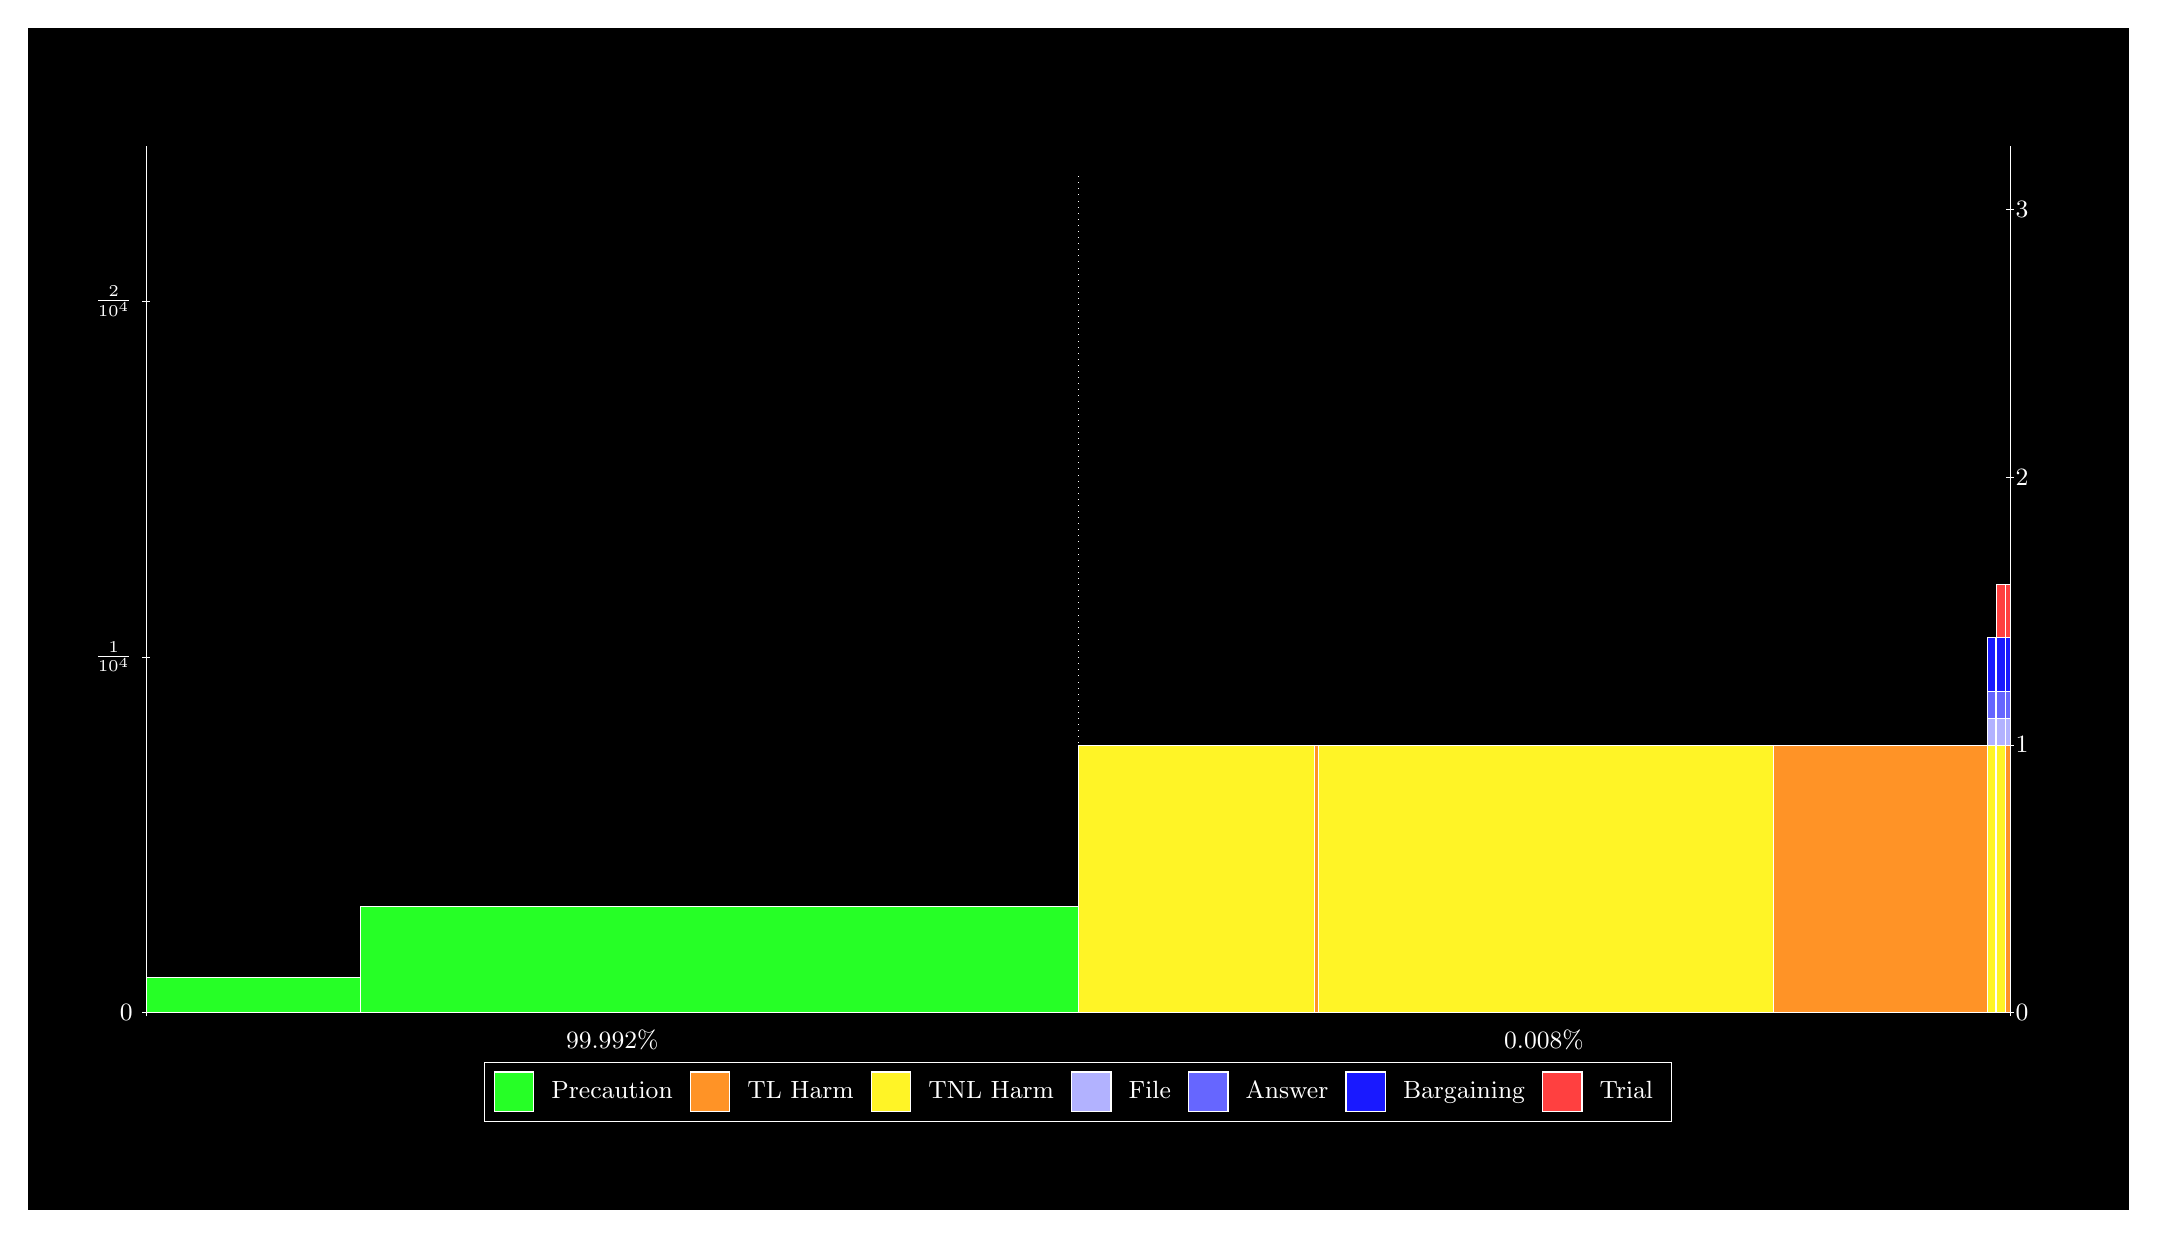
\begin{tikzpicture}
\draw[fill=black] (0,0) rectangle (26.667,15);
\draw[fill=green!85,draw=white,very thin] (1.5,2.5) rectangle (4.2218,2.9517);
\draw[fill=green!85,draw=white,very thin] (4.2218,2.5) rectangle (13.333,3.855);
\draw[fill=green!85,draw=white,very thin] (13.333,2.5) rectangle (16.338,2.5);
\draw[fill=yellow!85,draw=white,very thin] (13.333,2.5) rectangle (16.338,5.8991);
\draw[fill=green!85,draw=white,very thin] (16.338,2.5) rectangle (16.388,2.5);
\draw[fill=orange!85,draw=white,very thin] (16.338,2.5) rectangle (16.388,5.8991);
\draw[fill=green!85,draw=white,very thin] (16.388,2.5) rectangle (22.167,2.5001);
\draw[fill=yellow!85,draw=white,very thin] (16.388,2.5001) rectangle (22.167,5.8992);
\draw[fill=green!85,draw=white,very thin] (22.167,2.5) rectangle (24.876,2.5001);
\draw[fill=orange!85,draw=white,very thin] (22.167,2.5001) rectangle (24.876,5.8992);
\draw[fill=green!85,draw=white,very thin] (24.876,2.5) rectangle (24.984,2.5);
\draw[fill=yellow!85,draw=white,very thin] (24.876,2.5) rectangle (24.984,5.8991);
\draw[fill=blue!30,draw=white,very thin] (24.876,5.8991) rectangle (24.984,6.2391);
\draw[fill=blue!60,draw=white,very thin] (24.876,6.2391) rectangle (24.984,6.579);
\draw[fill=blue!90,draw=white,very thin] (24.876,6.579) rectangle (24.984,7.2588);
\draw[fill=green!85,draw=white,very thin] (24.984,2.5) rectangle (24.998,2.5);
\draw[fill=orange!85,draw=white,very thin] (24.984,2.5) rectangle (24.998,5.8991);
\draw[fill=blue!30,draw=white,very thin] (24.984,5.8991) rectangle (24.998,6.2391);
\draw[fill=blue!60,draw=white,very thin] (24.984,6.2391) rectangle (24.998,6.579);
\draw[fill=blue!90,draw=white,very thin] (24.984,6.579) rectangle (24.998,7.2588);
\draw[fill=green!85,draw=white,very thin] (24.998,2.5) rectangle (25.109,2.5);
\draw[fill=yellow!85,draw=white,very thin] (24.998,2.5) rectangle (25.109,5.8991);
\draw[fill=blue!30,draw=white,very thin] (24.998,5.8991) rectangle (25.109,6.2391);
\draw[fill=blue!60,draw=white,very thin] (24.998,6.2391) rectangle (25.109,6.579);
\draw[fill=blue!90,draw=white,very thin] (24.998,6.579) rectangle (25.109,7.2588);
\draw[fill=red!75,draw=white,very thin] (24.998,7.2588) rectangle (25.109,7.9386);
\draw[fill=green!85,draw=white,very thin] (25.109,2.5) rectangle (25.167,2.5);
\draw[fill=orange!85,draw=white,very thin] (25.109,2.5) rectangle (25.167,5.8991);
\draw[fill=blue!30,draw=white,very thin] (25.109,5.8991) rectangle (25.167,6.2391);
\draw[fill=blue!60,draw=white,very thin] (25.109,6.2391) rectangle (25.167,6.579);
\draw[fill=blue!90,draw=white,very thin] (25.109,6.579) rectangle (25.167,7.2588);
\draw[fill=red!75,draw=white,very thin] (25.109,7.2588) rectangle (25.167,7.9386);
\draw[white,very thin] (1.5,2.5) -- (1.5,13.5);
\draw[white,very thin] (1.45,2.5) -- (1.55,2.5);
\node[font=\small,text=white, anchor=east] at (1.45, 2.5) {0};
\draw[white,very thin] (1.45,7.0166) -- (1.55,7.0166);
\node[font=\small,text=white, anchor=east] at (1.45, 7.0166) {$\frac{1}{10^{4}}$};
\draw[white,very thin] (1.45,11.533) -- (1.55,11.533);
\node[font=\small,text=white, anchor=east] at (1.45, 11.533) {$\frac{2}{10^{4}}$};

\draw[white,dotted,very thin] (13.333,2.83) -- (13.333,13.17);
\draw[white,very thin] (25.167,2.5) -- (25.167,13.5);
\draw[white,very thin] (25.117,2.5) -- (25.217,2.5);
\node[font=\small,text=white, anchor=west] at (25.117, 2.5) {0};
\draw[white,very thin] (25.117,5.8991) -- (25.217,5.8991);
\node[font=\small,text=white, anchor=west] at (25.117, 5.8991) {1};
\draw[white,very thin] (25.117,9.2982) -- (25.217,9.2982);
\node[font=\small,text=white, anchor=west] at (25.117, 9.2982) {2};
\draw[white,very thin] (25.117,12.697) -- (25.217,12.697);
\node[font=\small,text=white, anchor=west] at (25.117, 12.697) {3};

\draw[white,very thin] (1.5,2.5) -- (25.167,2.5);
\draw[white,very thin] (1.5,2.45) -- (1.5,2.55);
\node[font=\small,text=white, anchor=north] at (1.5, 2.45) {};
\draw[white,very thin] (25.167,2.45) -- (25.167,2.55);
\node[font=\small,text=white, anchor=north] at (25.167, 2.45) {};

\node[font=\small,text=white,anchor=south] at (7.4167, 1.9) {99.992\%};
\node[font=\small,text=white,anchor=south] at (19.25, 1.9) {0.008\%};
\draw (13.3333,2.5) node (B) {};
\begin{scope}[align=center]
\matrix[scale=0.5,draw=white,below=0.5cm of B,nodes={draw},column sep=0.1cm]{
\node[rectangle,draw,minimum width=0.5cm,minimum height=0.5cm,fill=green!85]{}; & \node[draw=none,font=\small,text=white]{Precaution}; &
\node[rectangle,draw,minimum width=0.5cm,minimum height=0.5cm,fill=orange!85]{}; & \node[draw=none,font=\small,text=white]{TL Harm}; &
\node[rectangle,draw,minimum width=0.5cm,minimum height=0.5cm,fill=yellow!85]{}; & \node[draw=none,font=\small,text=white]{TNL Harm}; &
\node[rectangle,draw,minimum width=0.5cm,minimum height=0.5cm,fill=blue!30]{}; & \node[draw=none,font=\small,text=white]{File}; &
\node[rectangle,draw,minimum width=0.5cm,minimum height=0.5cm,fill=blue!60]{}; & \node[draw=none,font=\small,text=white]{Answer}; &
\node[rectangle,draw,minimum width=0.5cm,minimum height=0.5cm,fill=blue!90]{}; & \node[draw=none,font=\small,text=white]{Bargaining}; &
\node[rectangle,draw,minimum width=0.5cm,minimum height=0.5cm,fill=red!75]{}; & \node[draw=none,font=\small,text=white]{Trial}; \\\\
};\end{scope}

\end{tikzpicture}
\end{document}